\documentclass[12pt]{article}

\usepackage[utf8]{inputenc}
\usepackage[russian]{babel}
\usepackage{graphicx}
\usepackage{indentfirst}
\usepackage{booktabs}
\usepackage{amsmath}


\graphicspath{{pic/}}

\begin{document}

\begin{center}
	\LARGE 
	\textbf{Лабораторная работа 1}\\
	Вычисление определённых интегралов методом Монте-Карло\\
\end{center}

\begin{flushright}
	\large
	Игнашов Иван\\
	Вариант 8\\
\end{flushright}

\newpage

 \section*{1. Цель работы}
Изучение метода Монте-Карло, определение точности вычисления определенных интегралов методом Монте-Карло.

\subsection*{Порядок работы:}
\begin{enumerate}
	\item Записать математически анализируемую функцию 
		\begin{equation}
			f_{res} = \begin{cases}
						5*sin(2 \pi t) + 1 &t < 1\\
						5*sin(2 \pi (t-1)) + 1 &1 \le t \le 2\\
						2,5* \frac{2}{(t-2) + 1} &t > 2
					  \end{cases}
		\end{equation}
	\item Вычислить аналитически определенный интеграл $F = \int_0^3 f_{res}(t)dt$
	\item Разработать программу, вычисляющую величину F методом Монте-Карло при
заданном числе экспериментов
	\item При помощи разработанной программы вычислить определенный интеграл $\hat{F}$ %$\overset{^}{F}$
 при $N = 2^i$ экспериментах, где i = 0\dots14
\end{enumerate}

\newpage
 \section*{2. График функции $f_{res}(t)$}%
 \begin{figure}[!h]
	\centering
	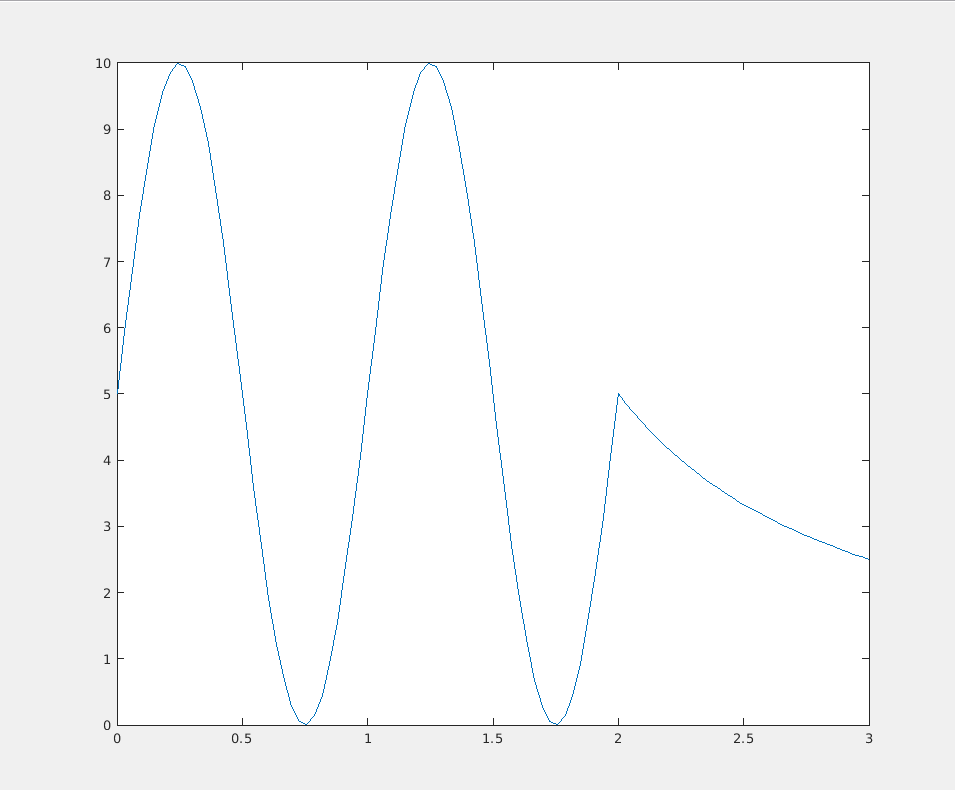
\includegraphics[width=\linewidth]{func_graph.png}
	\caption{График функции $f_{res}(t)$}
\end{figure}
Можно заметить, что на интересующей области $t = [0,3]$ функция принимает значения от 0 до 10
 
\newpage
 \section*{3. Аналитический расчет величины F}
Проинтегрируем кусочно-заданную функцию отдельно для каждого участка
\begin{center}
	\begin{tabular}[c]{lc|c|c}
  		& $f_1(t)$ & $f_2(t)$ & $f_3(t)$ \\[2mm]\hline
  		&&&\\
		Функция & $5*sin(2 \pi t) + 1$ & $5*sin(2 \pi (t-1)) + 1$ & $2,5* \frac{2}{(t-2) + 1}$\\
		&&&\\
		Неопр. интеграл & $5t - \frac{5cos(2 \pi t)}{2 \pi}$ & $5t - \frac{5cos(2 \pi t)}{2 \pi}$ & $5\log(t-1)$\\
		&&&\\
		Область & $0 \le t \le 1$ & $1 \le t \le 2$ & $2 \le t \le 3$\\
		&&&\\
		Значение & $5.0$ & $5.0$ & $3.46$\\\\
	\end{tabular}
\end{center}

Просуммировав получим $F = 13.46574$
 
\newpage
 \section*{4. Описание разработанной программы}
 %список использованных переменных, блок-схема, текст программы
 
\begin{figure}[!h]
	\centering
	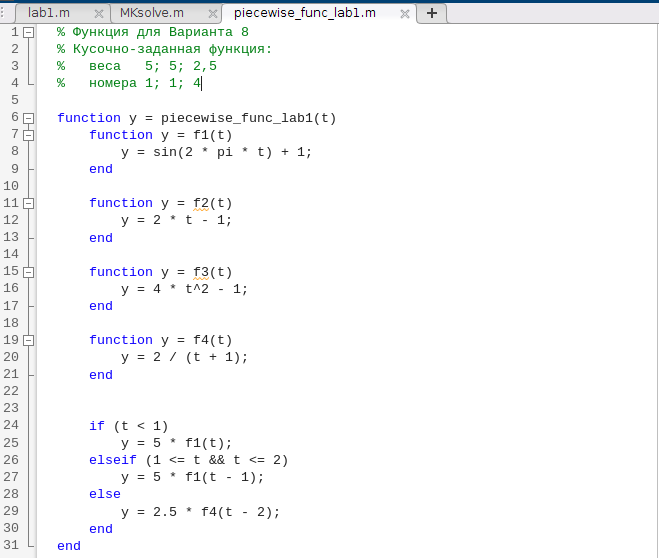
\includegraphics[width=\linewidth]{piecewise_func.png}
	\caption{Текст кусочно-заданной функции для Варианта 8}
\end{figure}
 
\begin{figure}[!h]
	\centering
	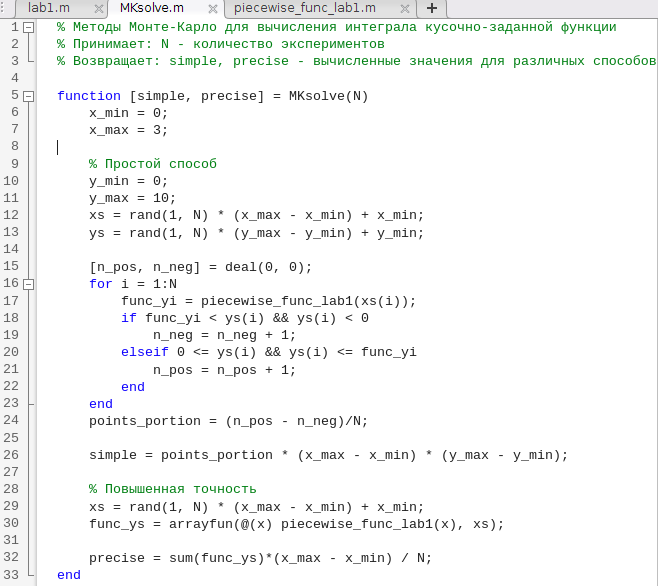
\includegraphics[width=\linewidth]{MKsolve.png}
	\caption{Текст функции вычисления интеграла}
\end{figure}

\begin{figure}[!h]
	\centering
	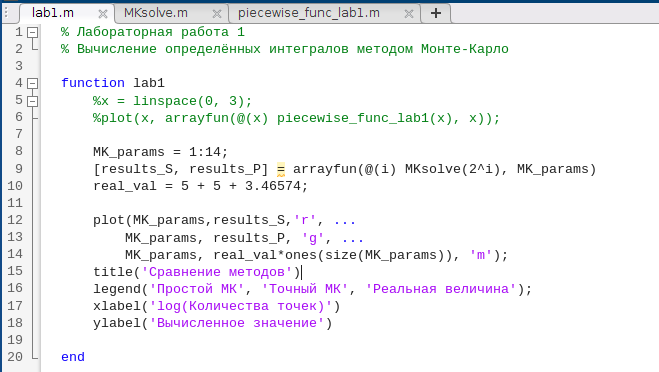
\includegraphics[width=\linewidth]{lab1.png}
	\caption{Текст процесса перебора экспериментов}
\end{figure}


 
\newpage
 \section*{5. Табличное представление результатов моделирования $F(N)$}
 
\begin{figure}[!h]
	\centering
	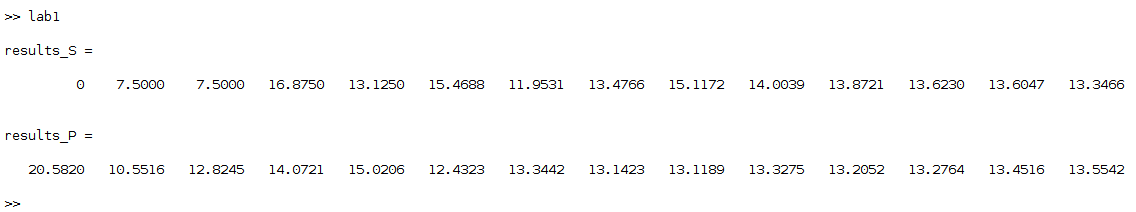
\includegraphics[width=\linewidth]{output.png}
	\caption{Вывод программы}
\end{figure}
Получим талицу значений для двух подходов:
\begin{center}
	\begin{tabular}[c]{lcccccccccccccc}
  		$2^i$ & 1 & 2 & 3 & 4 & 5 & 6 & 7 & 8 & 9 & 10 & 11 & 12 & 13 & 14\\[2mm]\hline
  		&&&\\
		Простой & 0.00 & 7.50 & 7.50 & 16.87 & 13.12 & 15.47 & 11.95 & 13.48 & 15.12 & 14.00 & 13.88 & 13.60 & 13.35\\
		&&&\\
		Точный & 20.58 & 10.55 & 12.82 & 14.07 & 15.02 & 12.43 & 13.14 & 13.12 & 13.33 & 13.20 & 13.27 & 13.45 & 13.55\\
		&&&\\
	\end{tabular}
\end{center}


\newpage
 \section*{6. График по рассчитанной таблице}
 
\begin{figure}[!h]
	\centering
	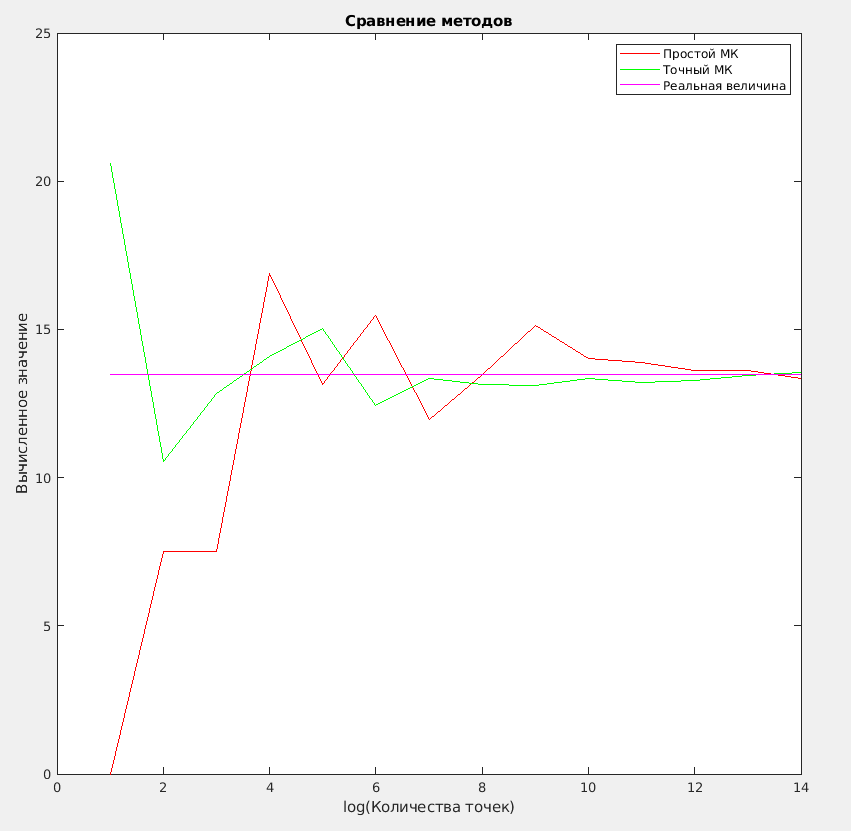
\includegraphics[width=\linewidth]{MK_compare_graph.png}
	\caption{Сравнение графиков методов}
\end{figure}

\newpage
 \section*{7. Выводы}
Целью данной лабораторной работы было изучение метода Монте-Карло и его применение. В процессе выполнения были реализованы 2 метода оценки интеграла функции: 

\begin{itemize}
	\item простой - основанный на площадях фигур
	\item с повышенной точностью - вычисление функции на случайных величинах $a_1\dots a_N$
\end{itemize}

На основе вывода программы были получены оценки инеграла функции двумя методами для различного количества случайных точек; построен график сравнения оценок с исходным, вычисленым аналитически, значением интеграла функции.

\end{document}